\documentclass{article}
\usepackage{latex-screenshot}
\usepackage{annotation} % Required for inserting images
\addbibresource{../../global_reference.bib}
\usetikzlibrary{patterns}
\newcolumntype{P}[1]{>{\centering\arraybackslash}p{#1}}%center table column elements
\newcolumntype{L}{>{\raggedright\arraybackslash}X}
\hfuzz=80pt
\hbadness=100000000
\begin{document}

\thispagestyle{empty}

\begin{center}
	\centering
	\vspace*{0.08\textheight}

	{\Large\textsc{x ray crystallography Proposal} \par}
	\vspace{0.9cm}
  {\LARGE DNA springs Project \par}
	\vspace{0.5cm}

	\vfill

  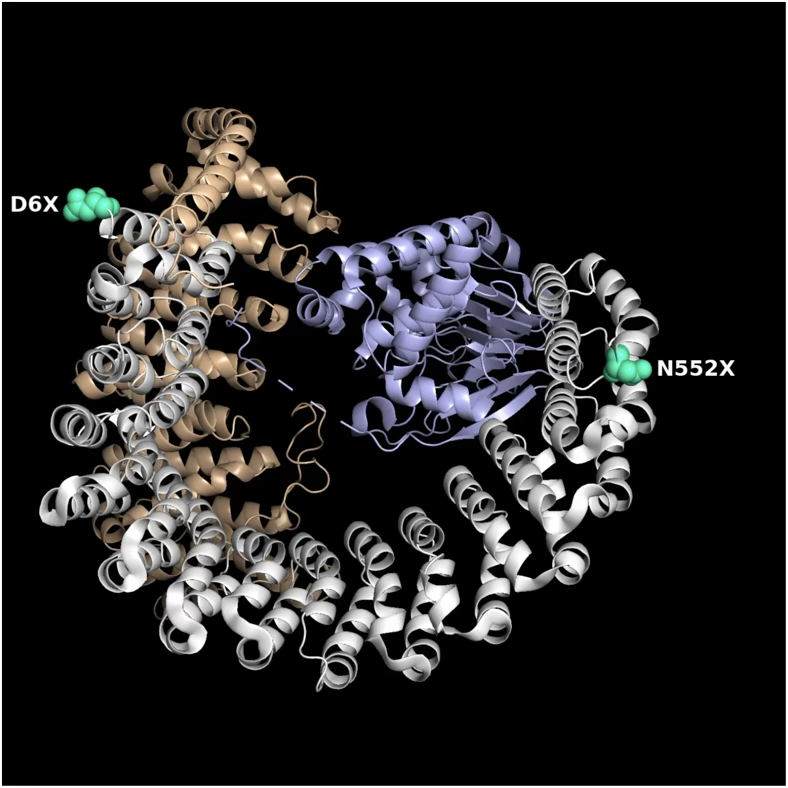
\includegraphics[width=0.3\textwidth]{assets/pp2a_attachmentPts.png}\par

	\vfill

	{\large Ian Poon\par}
	\vspace{0.35cm}
  {\normalsize September 2026 \par}
	\vspace{0.9cm}
\end{center}

\newpage

\tableofcontents
\newpage
\section{Proposal}
I would like to perform x ray crystallography experiments on sfGFP specifically I would like to obtain structural images sfGFP with tet attachments and their sfGFP chimeras variants

\section{objectives}
\begin{proposition}
to ascertain the proper attachment of ssDNA to sfGFP via our novel tet groups introduced via novel ncAA methods
\end{proposition}
DNA spring attachment via non cystine attachment points has never been done before on sfGFP. An validation of successful spring attachment beyond just a gel reading will most certainly pave the way for future usage of such click chemistry.

\begin{proposition}
to investigate the DNA spring forces applied to real proteins 
\end{proposition}
While the mechanics of DNA is well established how it actually trasmits forces to a real protein is not well established. At the resolution level of x ray crystallography, structural changes associated with spring attachment can be viewed and analyzed.

\begin{proposition}
to account for differences in fluroscence activity due to tet group and spring attachment
\end{proposition}
While there are no differences in emission/excitation wavelenghth, there is sufficient evidence of fluroscence intensity changes associated with addition of tet-groups and when springs are hybridized.


\section{justification}

\begin{fact}
we have established a reproducible inexpensive protocol for production of sfGFP chimeras at high thoroughputs required to xray crystallography
\end{fact}
Not only do we have concrete evidence of circular product on sfGFP, we were able to do so with extremely high purity without the use of HPLC.

\begin{fact}
We have observed differences in fluroscencent intensity as a result of DNA hybridization of chimera springs that is independent of concentration levels
\end{fact}

\begin{fact}
we have flurometer results on tet group quenching due to addition of tet groups \end{fact}

\begin{fact}
while the chimera can possibly be imaged using cryoEM(60kDa is on the low end), tet-attached sfGFP without DNA or WT sfGFP are definitively below the required size range for cryoEM imaging
\end{fact}

\begin{fact}
there are established protocols and experiments of x ray crystallography done on sfGFP already. 
\end{fact}


\section{additional justifcations}
First, a quick progress update on pp2a experiments. I am to report that I have also managed to obtain evidence of circular product reproducibly using an 80nt DNA spring.
\begin{figure}[H]
  \centering
  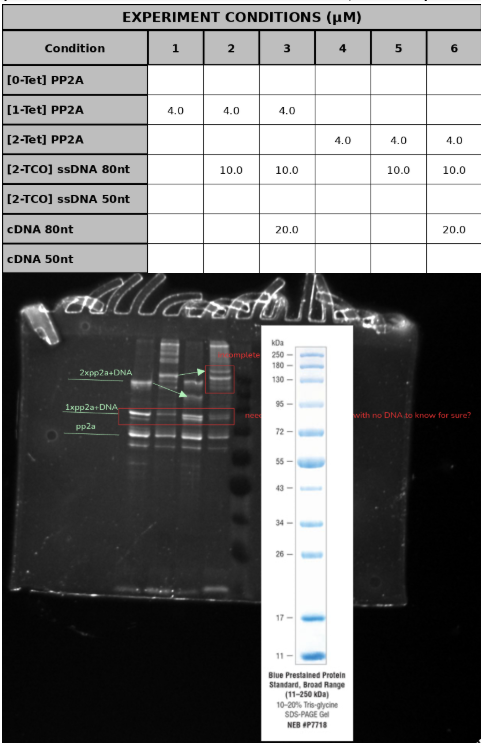
\includegraphics[width=0.49\textwidth]{assets/pp2aCHIM1.png}\hfill
  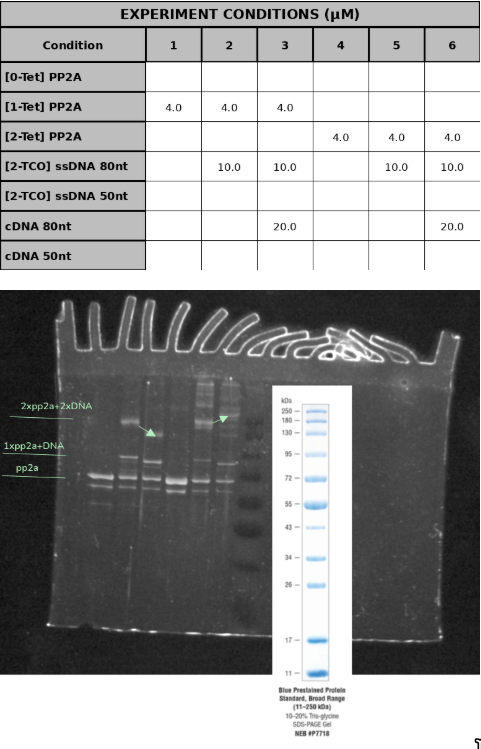
\includegraphics[width=0.49\textwidth]{assets/pp2aCHIM2.png}
  \caption{twice verified}
  \label{fig:pp2achim1}
\end{figure}
Refer to:
\begin{itemize}
  \item \href{https://hu.sharepoint.com/sites/sssc/hekstra_lab/_layouts/15/Doc.aspx?sourcedoc={13f23c5e-7b11-4dc7-96f7-e08c30f773b2}&action=edit&wd=target%28Notebook.one%7Cf0d88483-2b6e-4507-b41f-567d6de8172e%2F290909%20pp2a%204th%C2%A0time%7C2ec2f41b-539f-4f9b-9f80-3f39b2e5c750%2F%29&wdorigin=NavigationUrl}{290909 lab entry}
    \item \href{https://hu.sharepoint.com/sites/sssc/hekstra_lab/_layouts/15/Doc.aspx?sourcedoc={13f23c5e-7b11-4dc7-96f7-e08c30f773b2}&action=edit&wd=target%28Notebook.one%7Cf0d88483-2b6e-4507-b41f-567d6de8172e%2F260908%20pp2a%203rd%C2%A0%20time%7C8c7274d2-0d8d-46da-8119-9c74a7847716%2F%29&wdorigin=NavigationUrl}{260908 lab entry}
\end{itemize}
The next step likely involves purification as well as cryoEM imaging of the samples.

However Micheal is also involved in coursework and is understandably unable to train me on any new techniques or follow up on cryoEM at least until the end of the his qualification exams. So to lessen workload on Micheal and also not stall the spring project it might be best to consider this new direction if it makes sense.


Yes. There are several good X-ray crystallography papers on **superfolder GFP (sfGFP)**, including some that are unusually relevant to your project because they crystallized sfGFP with unnatural amino acids **at exactly \(Asp133\) and \(Asn149\)**, your two DNA-spring attachment regions.

\begin{table}[H]\noindent\begin{tabularx}{\linewidth}{LLLLL}
\hline
Paper & sfGFP construct & PDB & Resolution & Relevance \\ \hline
\textbf{Pédelacq et al., 2006} & Canonical sfGFP & \textbf{2B3P} & \textbf{1.40 \AA} & Reference sfGFP structure \\ \hline
\textbf{Dippel et al., 2016} & D133-pCNF, N149-pCNF, \textbf{D133/N149 double mutants} & \textbf{5DPG, 5DPH, 5DPI, 5DPJ} & 1.42--2.54 \AA & \textbf{Most relevant to your construct} \\ \hline
\textbf{Maurici et al., 2018} & D133-pNO\(_2\)F and N149-pNO\(_2\)F & \textbf{6DQ0, 6DQ1} & 2.05, 1.60 \AA & Also exactly your sites \\ \hline
Xia et al., 2013/14 & sfGFP W57A / W57G & \textbf{4LQT, 4LQU} & \textbf{1.10}, 1.60 \AA & Very high-resolution mutant structures \\ \hline
Olenginski et al., 2021 & ncAA substitutions at Y66 & \textbf{6B9C, 6OA8} & 1.70, \textbf{1.37 \AA} & Useful precedent for crystallizing genetically encoded ncAA-sfGFP \\ \hline
Heimsch et al., 2022 & redox-sensitive sfGFP variants & \textbf{7PCA, 7PCZ, 7PD0} & as high as \textbf{1.05 \AA} & Excellent high-resolution structural comparison \\ \hline
\end{tabularx}\end{table}

\subsubsection*{1. The canonical sfGFP crystal structure --- Pédelacq et al., 2006}

\textbf{Jean-Denis Pédelacq et al.}
\textbf{``Engineering and characterization of a superfolder green fluorescent protein.''}
\textbf{Nature Biotechnology 24, 79--88 (2006).}

This is the paper you should treat as the \textbf{baseline/reference structure for ordinary sfGFP}.

They determined the X-ray crystal structure of sfGFP, deposited as:

\textbf{PDB 2B3P --- 1.40 \AA{} resolution}

The paper explicitly used X-ray crystallography to understand why sfGFP folds more robustly than preceding GFP variants. \href{https://www.nature.com/articles/nbt1172}{\textbullet}

\href{https://www.nature.com/articles/nbt1172}{\textbullet}
\href{https://www.rcsb.org/structure/2B3P}{\textbullet}

For your future structural comparisons, \textbf{2B3P is probably the structure I would use as the primary WT-sfGFP reference.}

\subsubsection*{2. Most important for your project: Dippel et al., 2016}

\textbf{Dippel et al.}
\textbf{``Probing the effectiveness of spectroscopic reporter unnatural amino acids: a structural study.''}
\textbf{Acta Crystallographica D 72, 121--130 (2016).}
\textbf{DOI: 10.1107/S2059798315022858}

This is almost tailor-made for what you are doing.

They genetically incorporated unnatural amino acids into sfGFP at:

\begin{itemize}
    \item \textbf{\(Asp133\)}
    \item \textbf{\(Asn149\)}
    \item \textbf{\(Asp133 + Asn149\) simultaneously}
\end{itemize}

and then \textbf{actually solved their X-ray structures}. \href{https://pmc.ncbi.nlm.nih.gov/articles/PMC4756619/}{\textbullet}

The structures are:

\begin{table}[H]\noindent\begin{tabularx}{\linewidth}{LLL}
\hline
PDB & Modification & Resolution \\ \hline
\textbf{5DPG} & D133 \(\rightarrow\) p-cyano-Phe & \textbf{1.85 \AA} \\ \hline
\textbf{5DPH} & N149 \(\rightarrow\) p-cyano-Phe & \textbf{1.42 \AA} \\ \hline
\textbf{5DPI} & D133 + N149 \(\rightarrow\) p-cyano-Phe & \textbf{2.54 \AA} \\ \hline
\textbf{5DPJ} & D133 + N149 \(\rightarrow\) p-ethynyl-Phe & \textbf{2.50 \AA} \\ \hline
\end{tabularx}\end{table}

\href{https://www.rcsb.org/structure/5DPG}{\textbullet}

Most importantly, they directly compared these structures against \textbf{WT sfGFP 2B3P}. They found only small structural perturbations after ncAA incorporation. The paper describes D133 as a \textbf{solvent-exposed loop site}, whereas N149 is \textbf{partially buried on the \(\beta\)-barrel}. \href{https://pmc.ncbi.nlm.nih.gov/articles/PMC4756619/}{\textbullet}

\href{https://pmc.ncbi.nlm.nih.gov/articles/PMC4756619/}{\textbullet}
\href{https://www.rcsb.org/structure/5DPI}{\textbullet}
\href{https://www.rcsb.org/structure/5DPJ}{\textbullet}

\textbf{For your 2-Tet sfGFP, 5DPI and 5DPJ are particularly important controls.} They prove that sfGFP carrying \textbf{two bulky noncanonical amino acids simultaneously at essentially your two attachment positions can still crystallize and retain a near-native barrel structure.}

\subsubsection*{3. Maurici et al., 2018 --- independently crystallized D133 and N149 mutants}

\textbf{Maurici et al.}
\textbf{``Crystal structures of green fluorescent protein with the unnatural amino acid 4-nitro-L-phenylalanine.''}
\textbf{Acta Crystallographica F 74, 650--655 (2018).}
\textbf{DOI: 10.1107/S2053230X1801169X}

Again, the sites are \textbf{exactly D133 and N149}.

They used amber suppression to produce:

\textbf{D133-pNO\(_2\)Phe-sfGFP \(\rightarrow\) PDB 6DQ0 \(\rightarrow\) 2.05 \AA}

\textbf{N149-pNO\(_2\)Phe-sfGFP \(\rightarrow\) PDB 6DQ1 \(\rightarrow\) 1.60 \AA}

They aligned both against WT sfGFP and found only small RMS deviations, concluding that the substitutions caused little global structural disruption. \href{https://pubmed.ncbi.nlm.nih.gov/30279317/}{\textbullet}

\href{https://pmc.ncbi.nlm.nih.gov/articles/PMC6168768/}{\textbullet}
\href{https://www.rcsb.org/structure/6DQ0}{\textbullet}
\href{https://www.rcsb.org/structure/6DQ1}{\textbullet}

Their crystallization conditions are also useful experimentally. For example, the N149 construct was crystallized by \textbf{sitting-drop vapor diffusion} at roughly room temperature, with protein around \textbf{42 mg/mL}, and its diffraction was collected at 100 K. \href{https://pmc.ncbi.nlm.nih.gov/articles/PMC6168768/}{\textbullet}

\subsubsection*{4. Extremely high-resolution sfGFP mutants --- Xia et al.}

\textbf{Xia et al.}
\textbf{``The designability of protein switches by chemical rescue of structure: mechanisms of inactivation and reactivation.''}

They obtained several sfGFP mutant structures, including:

\textbf{4LQT --- W57A sfGFP --- 1.10 \AA}

\textbf{4LQU --- W57G sfGFP --- 1.60 \AA}

The 1.10 \AA 4LQT structure is exceptionally high resolution, so it can be useful if you want extremely precise reference values for backbone geometries, hydrogen-bond distances, side-chain positions, etc. \href{https://www.rcsb.org/structure/4LQT}{\textbullet}

\href{https://www.rcsb.org/structure/4LQT}{\textbullet}

I would still use \textbf{2B3P as the biologically appropriate WT reference}, rather than 4LQT, because W57A itself alters sfGFP.

\subsubsection*{5. ncAA-containing sfGFP crystallography --- Olenginski et al., 2021}

\textbf{Olenginski et al.}
\textbf{``Structural and spectrophotometric investigation of two unnatural amino-acid altered chromophores in the superfolder green fluorescent protein.''}
\textbf{Acta Crystallographica D 77, 1010--1018 (2021).}

Structures:

\begin{itemize}
    \item \textbf{6B9C} --- Y66 nitrophenylalanine sfGFP --- \textbf{1.70 \AA}
    \item \textbf{6OA8} --- Y66 cyanophenylalanine sfGFP --- \textbf{1.37 \AA}
\end{itemize}

They used molecular replacement with \textbf{2B3P} as the starting sfGFP model. \href{https://pmc.ncbi.nlm.nih.gov/articles/PMC8329867/}{\textbullet}

\href{https://pmc.ncbi.nlm.nih.gov/articles/PMC8329867/}{\textbullet}

This provides further evidence that \textbf{GCE-produced ncAA-containing sfGFP is perfectly compatible with conventional protein crystallography}.

\subsubsection*{The key finding for your sfGFP DNA-spring work}

The literature situation is actually better than I expected because \textbf{your D133/N149 region has already been extensively studied crystallographically}.

In particular, Dippel et al. crystallized a \textbf{D133/N149 double-ncAA sfGFP}. That makes \textbf{5DPI/5DPJ probably the closest existing structural analog to your 2-Tet sfGFP before DNA conjugation}. \href{https://www.rcsb.org/structure/5DPI}{\textbullet}

There is, however, an important distinction:

\textbf{I have not found an X-ray structure in these searches of sfGFP containing Tet2-Et specifically at both D133/N149, nor of an sfGFP--DNA circular spring chimera.} The closest structures substitute other aromatic ncAAs at these same sites.

So for the experiment we were discussing yesterday, the ideal structural series would be:

\textbf{2B3P WT sfGFP \(\rightarrow\) your 2-Tet D133/N149 sfGFP \(\rightarrow\) 2-Tet sfGFP + attached ssDNA \(\rightarrow\) 2-Tet sfGFP + hybridized dsDNA spring.}

The first structure already exists; remarkably, \textbf{very close analogues of the second also already exist}.

If your aim is to determine whether an \textbf{\(\sim\)50-bp spring mechanically changes backbone geometry around D133/N149 and ultimately the chromophore/H148 region}, the Dippel 2016 paper is the one I would read first. It gives you a very strong crystallographic control separating \textbf{``structural changes caused merely by ncAA substitution''} from changes you might later attribute to the DNA spring.

\printbibliography
\end{document}

